\chapter{Results}
\label{chapterlabel5}

In this chapter I offer the results of the analysis conducted in this research project. I will begin by providing background context for each of our selected case studies. I then summarize the characteristics of the data produced in each case study and provide an overview of the dynamics of data production over the duration of each mapping campaign. I will present results that demonstrate the prevalence of data maintenance following each campaign. 

\section{Case study context}

Prior to providing the empirical results of our analysis, I briefly address the humanitarian context in each of our case studies and their relevance to the humanitarian mapping community. The geographic location and spatial distribution of mapping activity for each case study can be seen in Figure \ref{fig:map}. Full-size versions of each inset map can be found in Appendix \ref{appendixlabel1}. 

%%%%%%%%%%%%%%%%%%%%%%%%%% Over time image 
\begin{figure} % opens the figure environment. the '[H]' forces the image to be Here
    \centering % puts the image in the horizontal centre of the page
    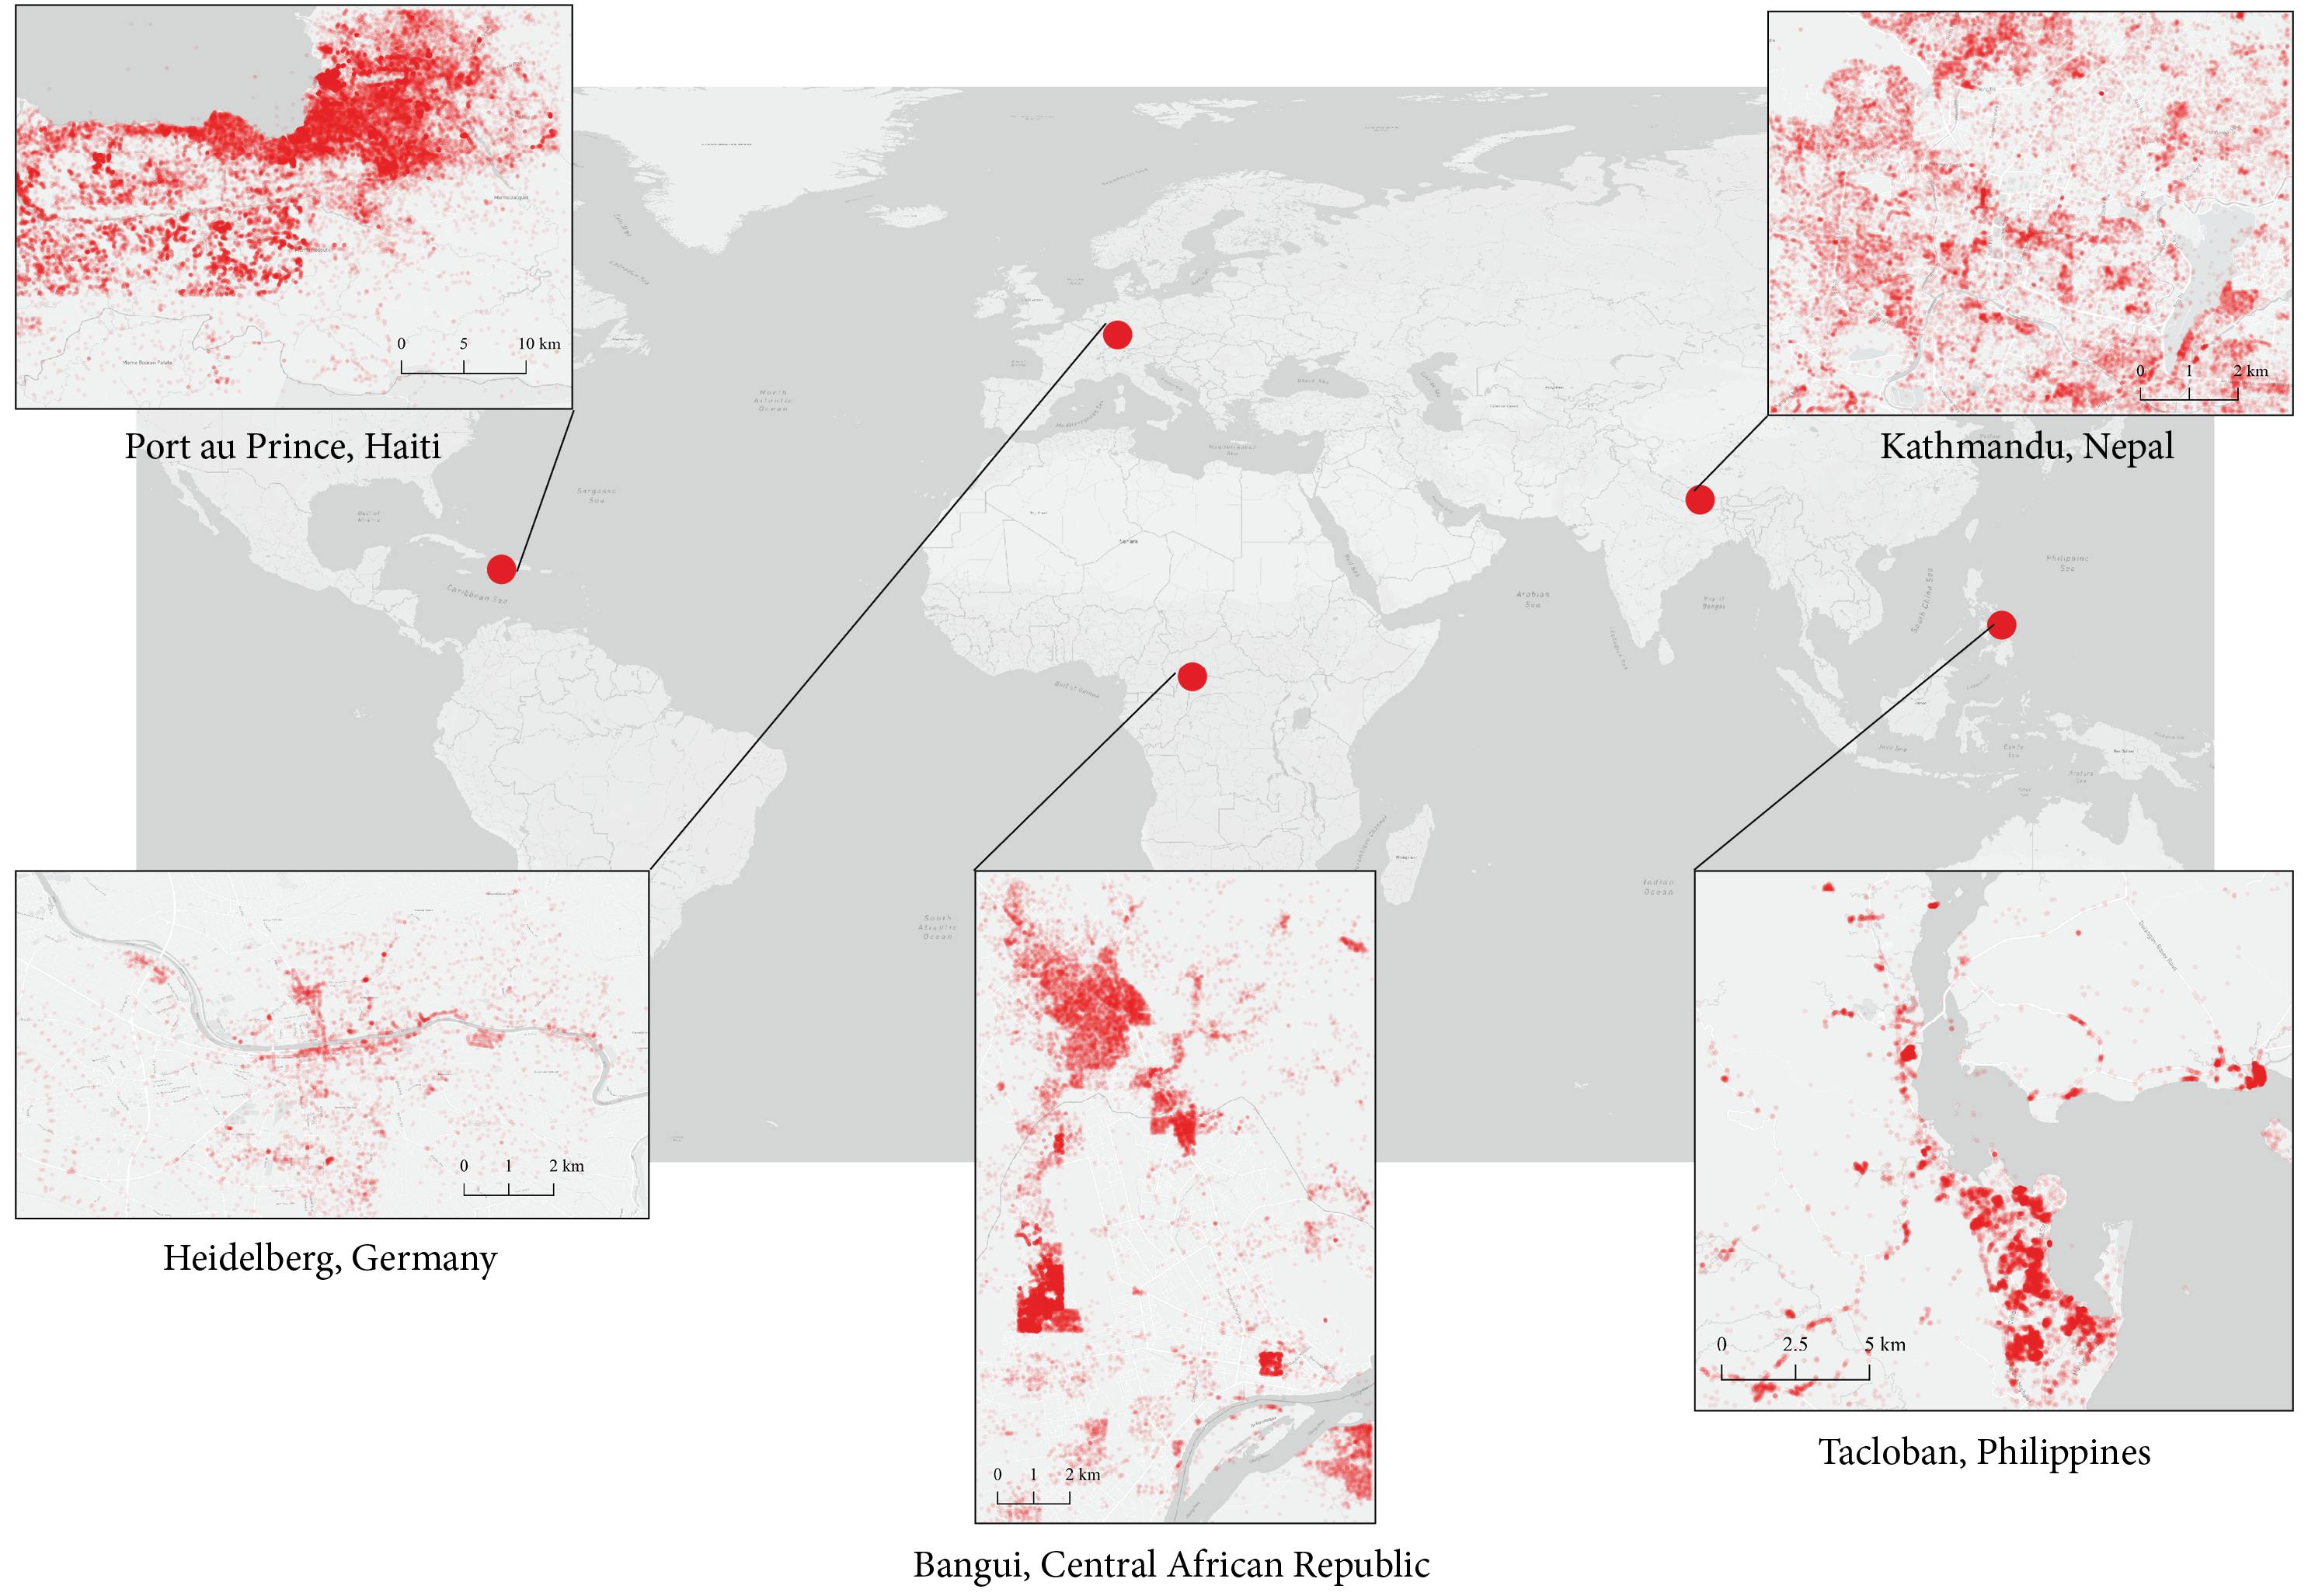
\includegraphics[width = \textwidth]{Images/sum_map.png} %this tells latex what graphics to include. 
    \caption[Map of case study locations and spatial distribution of features added.]{Map of case study locations and spatial distribution of features added. Greater intensity of colour corresponds to a greater density of features added to OSM during each mapping campaign.} % this prints the caption below the figure
    \label{fig:map} % this internally labels the figure for future referencing.
\end{figure}
%%%%%%%%%%%%%%%%%%%%%%%%%% 

\subsection{Port au Prince, Haiti}

Haiti experienced a magnitude 7.0 earthquake on January 12, 2010, which caused an estimated 300,000 deaths, and widespread building damage and population displacement \parencite{desroches_overview_2011}. The effects of the earthquake were further exacerbated by an outbreak of cholera in October 2010 that spread to informal settlements \parencite{human_rights_watch_world_2011}. It is estimated that this event has caused USD \$8.1bn damage \parencite{cavallo_estimating_2010}. Humanitarian mapping efforts in Haiti following this earthquake have been well researched and discussed in past academic literature \parencite{zook_volunteered_2010, soden_crowdsourced_2014, palen_success_2015, meier_crisis_2012}. This disaster has been described as a "catalyzing event" for many digitally-focused volunteer communities \parencite[p. 314]{soden_crowdsourced_2014}. Mapping efforts around this event also led to the formalization of the Humanitarian OpenStreetMap Team (HOT), the process of which is described in further detail by \textcite{soden_crowdsourced_2014}. Throughout their post-disaster efforts to raise awareness of the value of OSM and mobilize a community of mappers, one of HOT's primary goals was to "embed" OSM within the local community and further local ownership of this data. This effort was intended to allow for the long-term use of OSM data beyond this humanitarian response \parencite{soden_crowdsourced_2014}. As shown by Figure \ref{fig:map}, the features mapped within this study area are largely clustered around the coast of Port au Prince. 

\subsection{Tacloban, Philippines}

The Philippines was greatly impacted by a tropical cyclone, Typhoon Haiyan (or Typhoon Yolanda), on November 8, 2013. This typhoon is said to be one of the strongest ever recorded \parencite{lum_typhoon_2014}. USAID estimates that this disaster has caused over 6,000 deaths and the destruction or damage of over 1 million homes \parencite{noauthor_typhoon_2014}. The city of Tacloban was one of the areas that faced greatest impact and was thus where much relief effort was focused \parencite{lum_typhoon_2014}, as shown by the clustering of features on the inset map in Figure \ref{fig:map}. Following this crisis, mapping efforts in OSM were coordinated by HOT, with high-volume, remote mapping efforts organized by the newly developed Tasking Manager \parencite{openstreetmap_wiki_wikiproject_2018}. \textcite{palen_success_2015} note that the mapping efforts in the Philippines were facilitated by these new tools for technical collaboration, which incorporated lessons learned from previous humanitarian mapping efforts, such as in Haiti. Details from the OSM Wiki page indicate that most mapping efforts were focused on buildings, roads, and infrastructure damage \parencite{openstreetmap_wiki_wikiproject_2018}.

\subsection{Kathmandu, Nepal}

Nepal was hit with a magnitude 7.6 earthquake on April 25th, centered approximated 76 km northwest of Kathmandu, which was followed by over 300 aftershocks of over 4.0 magnitude \parencite{noauthor_nepal_2015}. It is estimated that over 9,000 people died in these disasters and over half a million homes were destroyed or damaged \parencite{noauthor_nepal_2015}. The major earthquake and its aftershocks caused further disasters such as landslides and avalanches, and exacerbated vulnerabilities to flooding in many areas \parencite{noauthor_nepal_2015}. As is described by \textcite{soden_infrastructure_2016} this crisis can be viewed as a turning point in the history of post-disaster mapping in the OSM community. Whereas in the Haiti case where HOT needed to conduct notable outreach to spread awareness of the applicability of OSM data, interviews with GIS practitioners in the field found that up-to-date OSM data came to be an "expected resource" in Nepal \parencite[p. 2801]{soden_infrastructure_2016}. Figure \ref{fig:map} shows how the mapping activity is decentralized throughout our study area of Kathmandu.

\subsection{Bangui, Central African Republic}

Violence and instability in CAR mounted in March 2013 when the Seleka rebel group seized the capital city, Bangui \parencite{global_conflict_tracker_violence_2020}. This event launched a humanitarian mapping campaign that aimed to provide baseline geospatial data for the country \parencite{openstreetmap_wiki_wikiproject_2020}. Mapping the country's road network was a priority of this campaign, as well as mapping affected cities and towns, as identified by local humanitarian stakeholders \parencite{openstreetmap_wiki_wikiproject_2020}. The features mapped within our study area in Bangui are clustered within the periphery of the area, as shown in Figure \ref{fig:map}. UNICEF data for health facilities, water points, and schools was also imported as part of this campaign \parencite{openstreetmap_wiki_wikiproject_2020}.

\subsection{Heidelberg, Germany}

Heidelberg serves as our reference case study, allowing us to compare humanitarian mapping activities with those from a part of the map that has been established as high quality (researched by \textcite{arsanjani_assessing_2013} and previously applied as a reference case study by \textcite{anderson_crowd_2018}). While I generalize and refer to all of our case studies as "mapping campaigns", I acknowledge that this Heidelberg case does not refer to a distinct campaign, as with our other humanitarian case studies. Figure \ref{fig:map} shows how the features mapped in this case study are distributed around the centre of our study area.

\section{Characteristics of OSM data production}

In this section, I provide details of the data that was produced in each of our case studies.

%%%%%%%%%%%%%%%%%%%%%%%%%% TABLE - summary
\begin{table}[H]
\centering
\caption{Summary statistics for data produced in each case study.}
\label{tab:summary}
\begin{tabular}{lllllll} 
\toprule
Case Study     & \begin{tabular}[c]{@{}l@{}}Duration\\$Days$\end{tabular} & \begin{tabular}[c]{@{}l@{}}Area\\$km^2$\end{tabular} & \begin{tabular}[c]{@{}l@{}}Unique \\Contributors\end{tabular} & \begin{tabular}[c]{@{}l@{}}Features\\Created\end{tabular} & Burst & Style    \\ 
\midrule
Port au Prince & 658                                                      & 1397                                                 & 313                                                           & 31962                                                     & 17    & event    \\
Tacloban       & 82                                                       & 356                                                  & 199                                                           & 19801                                                     & 1     & event    \\
Kathmandu      & 250                                                      & 98                                                   & 881                                                           & 37587                                                     & 5     & event    \\
Bangui         & 1012                                                     & 203                                                  & 170                                                           & 36788                                                     & 164   & mission  \\
Heidelberg     & 365                                                      & 192                                                  & 108                                                           & 3786                                                      & 146   & mission  \\
\bottomrule
\end{tabular}
\end{table}
%%%%%%%%%%%%%%%%%%%%%%%%%% 

Table \ref{tab:summary} provides a basic summary of the data produced in each case study. I see that each case study covers varying temporal and spatial extents. The mapping campaign in Bangui, for example, is over ten times longer than that in Tacloban. The mapping campaign in Port au Prince covers an area that is nearly 15 times larger than that in Kathmandu. Despite these differences, all humanitarian mapping campaigns have produced volumes of data that are of the same order of magnitude (approximately 20,000 to 40,000 new features created). The reference case study in Heidelberg has produced notably less data. The case study in Kathmandu stands out when considering the number of unique contributors (nearly three-times the case study with the next largest number), and the density of contributors over space. The burstiness value, which corresponds to the number of days until 50\% of all the data from the campaign has been created, for each case study results in the ‘style’ classification \parencite{dittus_mass_2017}. Both Bangui and Heidelberg are classified as "missions", while Port au Prince, Tacloban, and Kathmandu are "events". 

%%%%%%%%%%%%%%%%%%%%%%%%%% Over time image 
\begin{figure} % opens the figure environment. the '[H]' forces the image to be Here
    \centering % puts the image in the horizontal centre of the page
    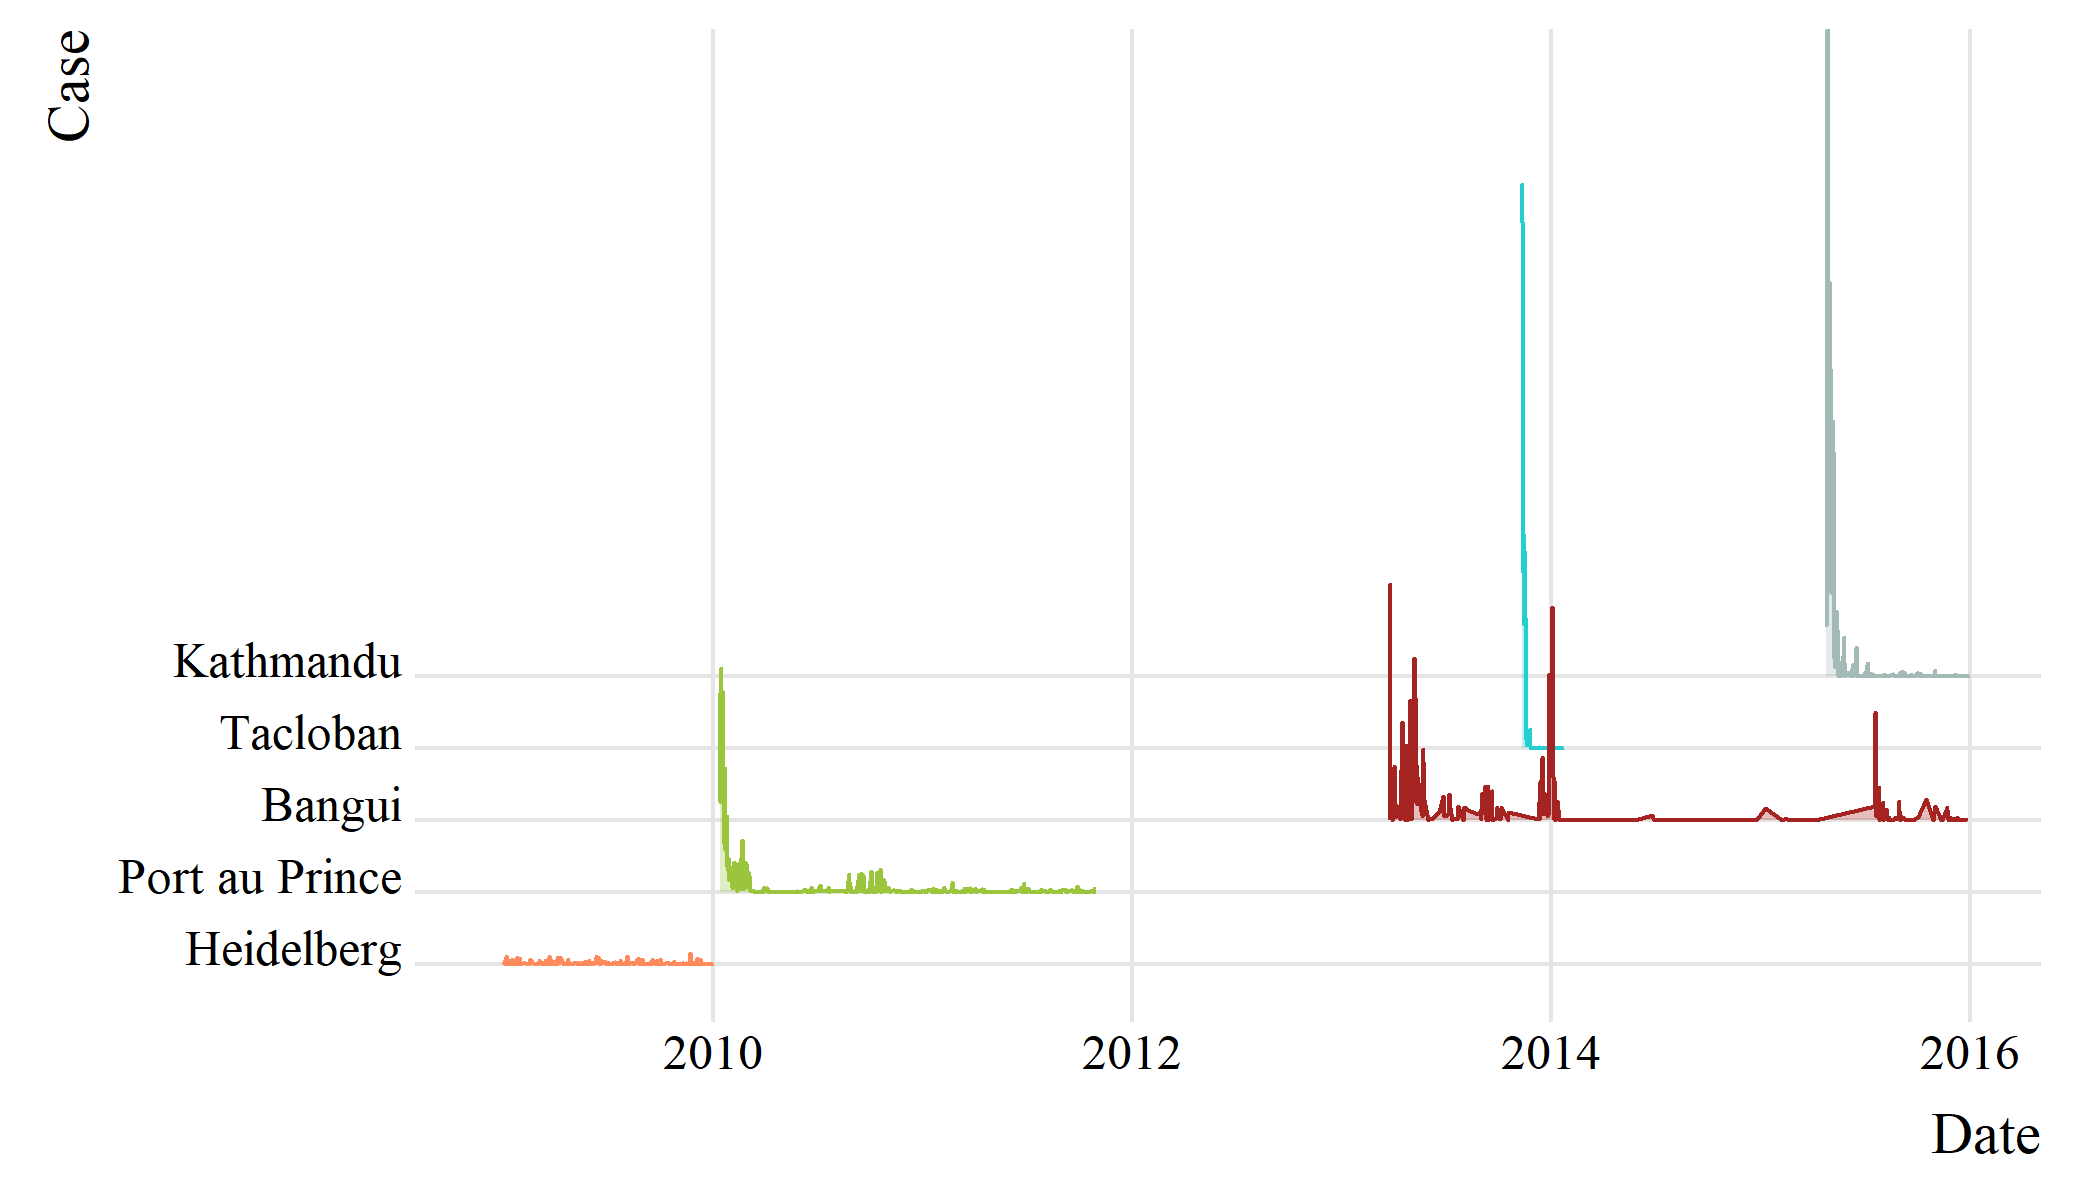
\includegraphics[width = \textwidth]{Images/overtime.png} %this tells latex what graphics to include. 
    \caption[Daily volume of OSM contributions throughout duration of each mapping campaign.]{Daily volume of OSM contributions throughout duration of each mapping campaign. The implied z-axis indicates the relative daily contribution volume.} % this prints the caption below the figure
    \label{fig:time} % this internally labels the figure for future referencing.
\end{figure}
%%%%%%%%%%%%%%%%%%%%%%%%%% 

The dynamics of contributing patterns for each case study are further demonstrated in Figure \ref{fig:time}, which shows the daily magnitude of contributions for each mapping campaign. The campaigns in Tacloban, Port au Prince, and Kathmandu exhibit the characteristics of event-style campaigns, as described by \textcite{dittus_mass_2017}, whereby mapping activity is front-loaded and decays quickly after the beginning of the campaign. The magnitude of early mapping efforts in Tacloban, Kathmandu, and Port au Prince, shown by the burstiness values from Table \ref{tab:summary} and the size of the peaks in Figure \ref{fig:time}, set these cases apart from others. The mapping in Bangui and the Heidelberg reference show a pattern where activity is more evenly sustained over a longer period of time. 

Further differences between the two mapping campaign styles are shown in Figure \ref{fig:scatter}, where I see that the ‘event-style’ campaigns have a stronger relationship between the number of daily contributors and contributions.  In all cases, however, the relationship between daily contributor volume and daily contribution volume is statistically significant. Heidelberg and Bangui, the two ‘mission-style’ campaigns, have a notably shorter range of daily unique contributors (no more than 10 in a day), while campaigns such as that in Kathmandu have reached over 150 unique contributors in a day. 

%%%%%%%%%%%%%%%%%%%%%%%%%% Scatter image
\begin{figure} % opens the figure environment. the '[H]' forces the image to be Here
    \centering % puts the image in the horizontal centre of the page
    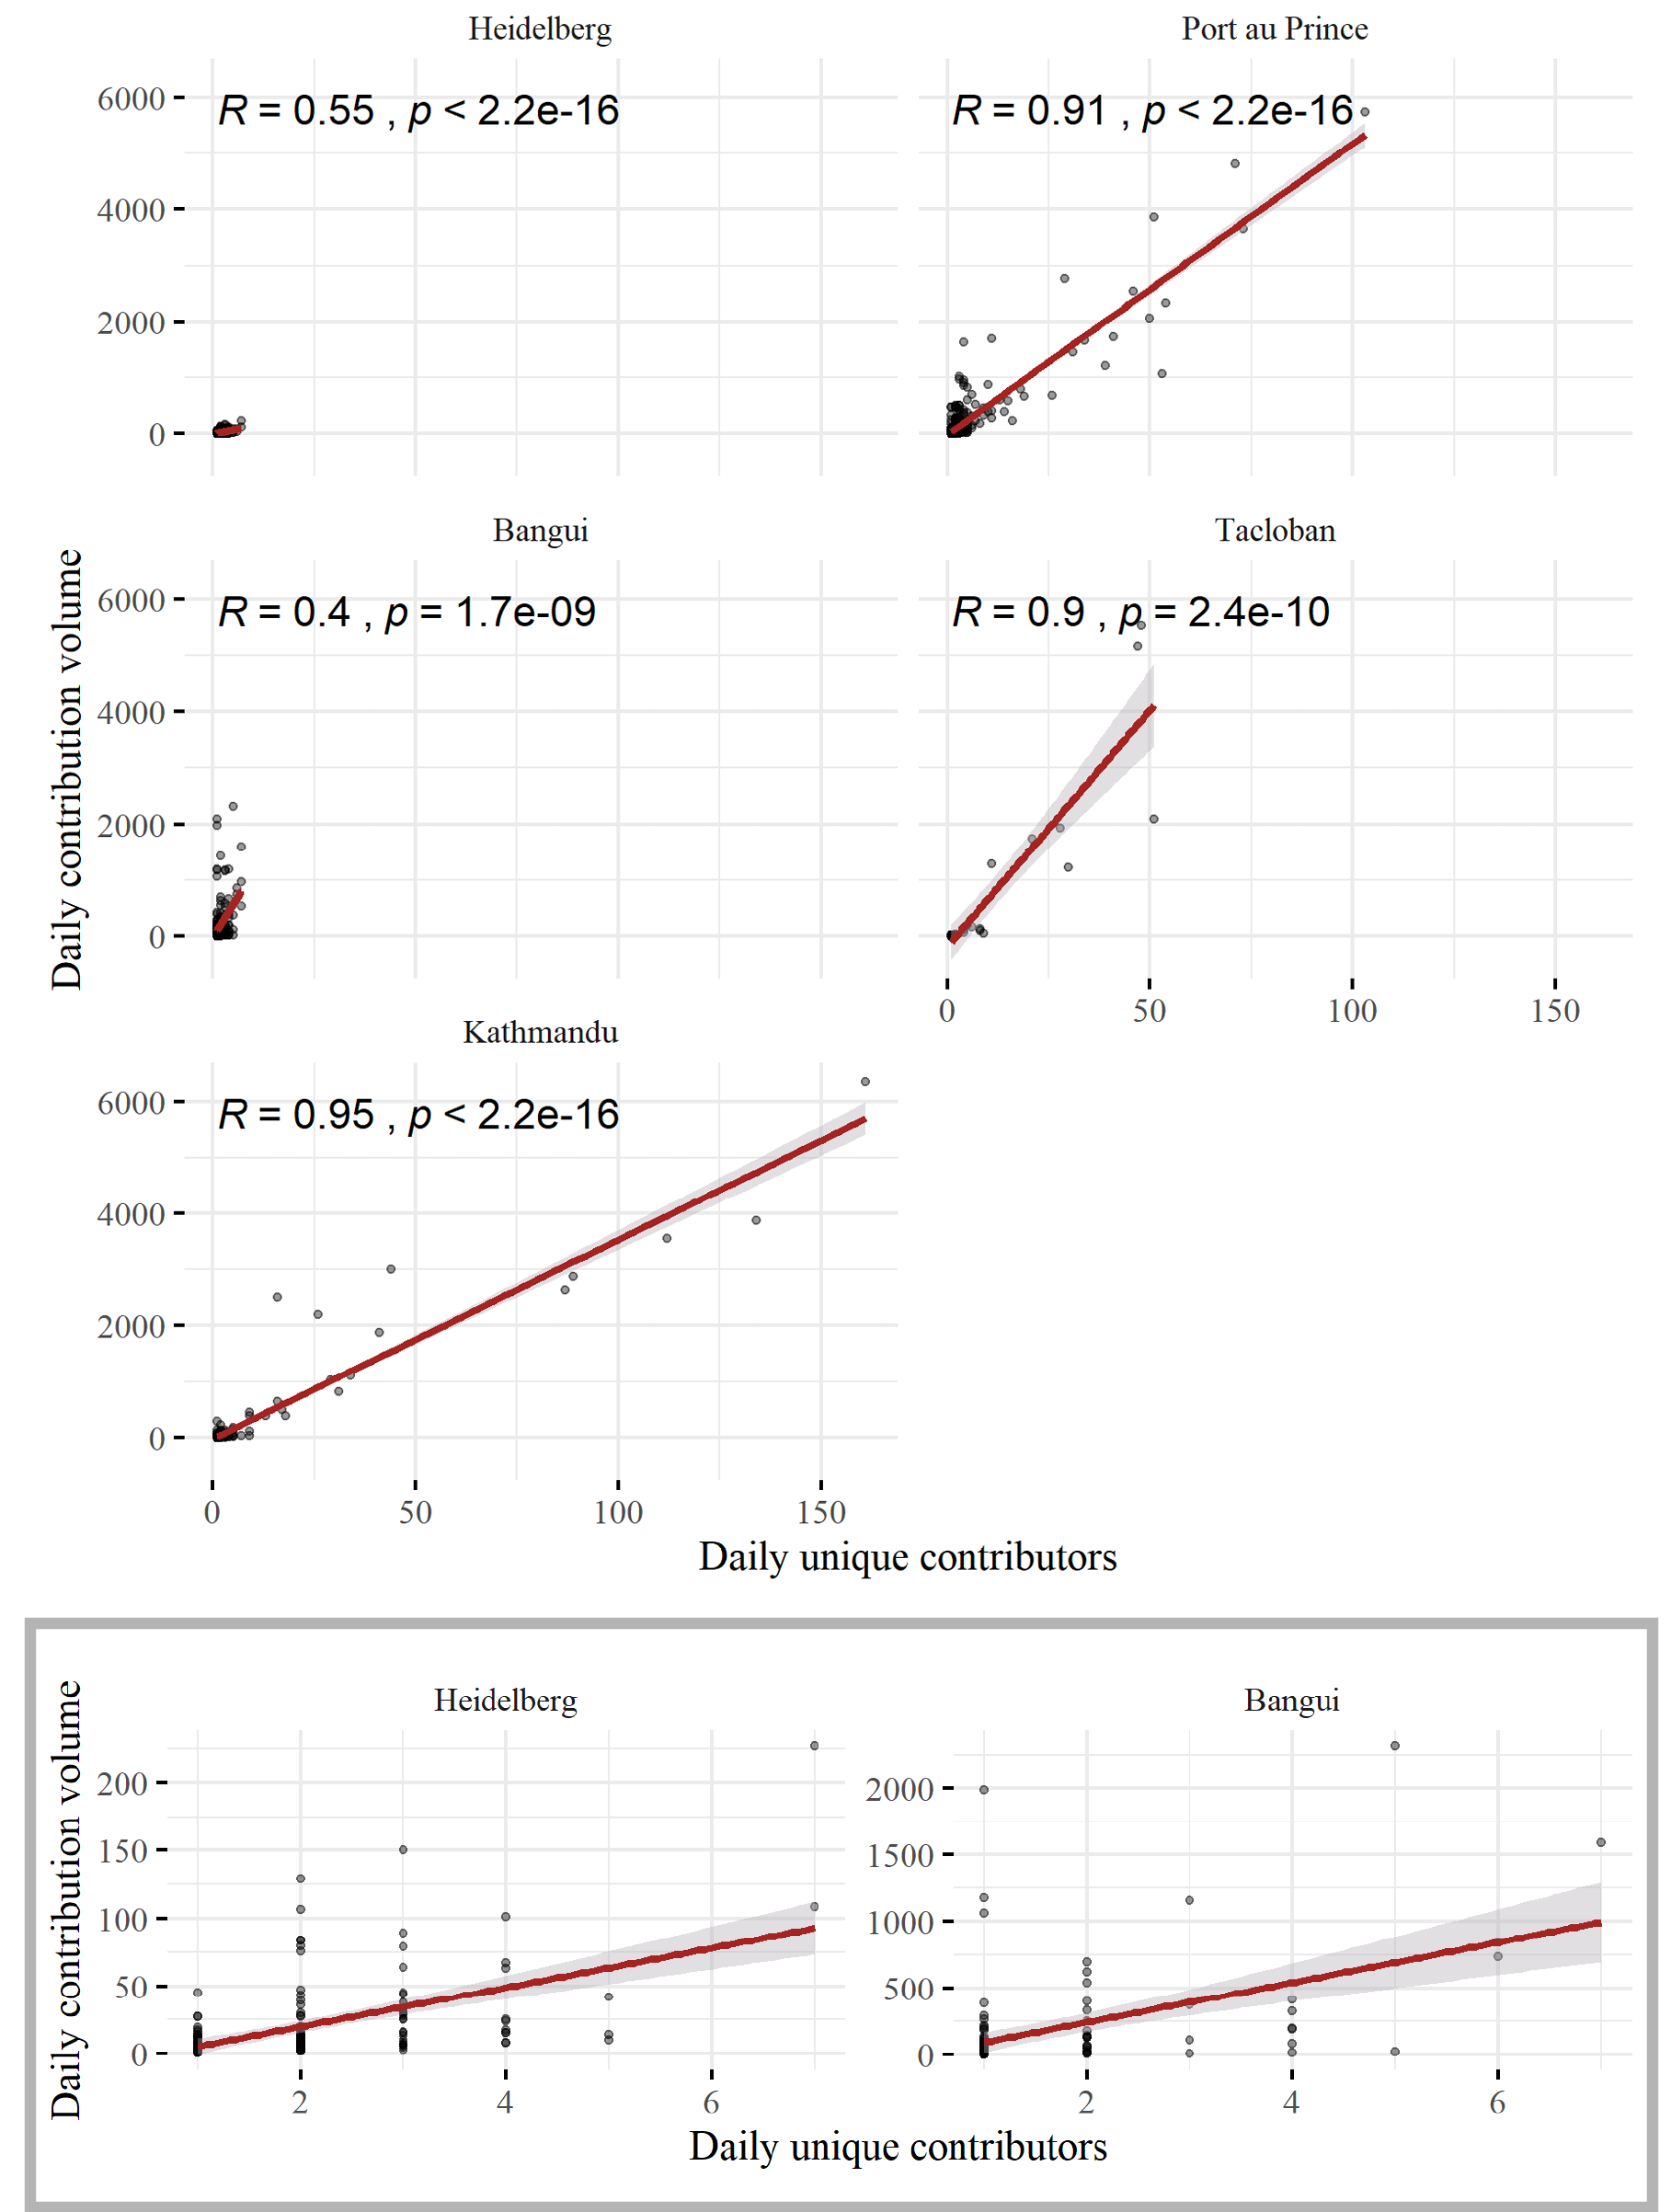
\includegraphics[width = \textwidth]{Images/scatter_inset.png} %this tells latex what graphics to include. 
    \caption[Scatterplots of daily unique contributors against daily contribution volume.]{Scatterplots of daily unique contributors against daily contribution volume (in number of contributions) for each mapping campaign. Includes inset of Heidelberg and Bangui with rescaled axes.} % this prints the caption below the figure
    \label{fig:scatter} % this internally labels the figure for future referencing.
\end{figure}
%%%%%%%%%%%%%%%%%%%%%%%%%% 

Both Figures \ref{fig:time} and \ref{fig:scatter} show a clear difference in the daily volume of data contributed between the Heidelberg reference and the humanitarian campaigns.  Daily contribution volume in Heidelberg during this time barely exceed 100 new features, while humanitarian campaigns such as those in Tacloban and Kathmandu reach over 4,000 and 6,000 new features in a day, respectively, at their peaks. 

Table \ref{tab:tags}, below, provides insight into the type of data that is contributed in each mapping campaign. I see similarities across all cases as the \texttt{building}, \texttt{highway}, and \texttt{source} tags are frequently occurring in each. The humanitarian campaigns show crisis-specific tags, such as \texttt{typhoon:damage} and \texttt{damage:event}.  

Table \ref{tab:sources} provides insight into the data sources for each mapping campaign. For the humanitarian cases, I see that a notable proportion of the data was generated from satellite imagery (eg. Bing or Worldview), suggesting that many of the contributors are remotely located. Very little of the Heidelberg data has been tagged with a source, however none of the sources listed are from satellite imagery, so I can perhaps infer that much of this data was added by local contributors. 

%%%%%%%%%%%%%%%%%%%%%%%%%% TABLE - tags 
\begin{table}[H]
\centering
\caption[Frequently occurring tag keys.]{Top five most frequently occurring tag keys across each case study. Keys highlighted in grey appear across at least 4/5 case studies.}
\label{tab:tags}
\begin{tabular}{@{} llll @{}} 
\toprule
Port au Prince                               &                  & Tacloban                                     &                   \\ 
\midrule
\textit{key}                                 & \textit{percent} & \textit{key}                                 & \textit{percent}  \\
{\cellcolor[rgb]{0.875,0.875,0.875}}source   & \Chart{0.76}             & {\cellcolor[rgb]{0.875,0.875,0.875}}building & \Chart{0.89}              \\
{\cellcolor[rgb]{0.875,0.875,0.875}}highway  & \Chart{0.33}             & {\cellcolor[rgb]{0.875,0.875,0.875}}source   & \Chart{0.27}              \\
{\cellcolor[rgb]{0.875,0.875,0.875}}building & \Chart{0.29}             & typhoon:damage                               & \Chart{0.11}                \\
attribute\_source\_date                      & \Chart{0.17}             & {\cellcolor[rgb]{0.875,0.875,0.875}}highway  & \Chart{0.27}               \\
name                                         & \Chart{0.11}             & typhoon:damaged                              & \Chart{0.15}               \\ 
\toprule
Bangui                                       &                  & Kathmandu                                    &                   \\ 
\midrule
\textit{key}                                 & \textit{percent} & \textit{key}                                 & \textit{percent}  \\
{\cellcolor[rgb]{0.875,0.875,0.875}}building & \Chart{0.58}             & {\cellcolor[rgb]{0.875,0.875,0.875}}building & \Chart{0.74}              \\
{\cellcolor[rgb]{0.875,0.875,0.875}}source   & \Chart{0.35}               & {\cellcolor[rgb]{0.875,0.875,0.875}}source   & \Chart{0.24}              \\
{\cellcolor[rgb]{0.875,0.875,0.875}}highway  & \Chart{0.11}             & idp:camp\_site                               & \Chart{0.14}              \\
source:date                                  & \Chart{0.06}              & damage:event                                 & \Chart{0.13}              \\
project:eurosha\_2012                        & \Chart{0.06}              & {\cellcolor[rgb]{0.875,0.875,0.875}}highway  & \Chart{0.04}               \\ 
\toprule
Heidelberg                                   &                  &                                              &                   \\ 
\midrule
\textit{key}                                 & \textit{percent} &                                              &                   \\
{\cellcolor[rgb]{0.875,0.875,0.875}}highway  & \Chart{0.46}             &                                              &                   \\
name                                         & \Chart{0.23}               &                                              &                   \\
tracktype                                    & \Chart{0.14}             &                                              &                   \\
created\_by                                  & \Chart{0.13}             &                                              &                   \\
amenity                                      & \Chart{0.10}              &                                              &     \\
\bottomrule
\end{tabular}
\end{table}
%%%%%%%%%%%%%%%%%%%%%%%%%%

%%%%%%%%%%%%%%%%%%%%%%%%%% TABLE - sources
\begin{table}[H]
\centering
\caption[Frequently occurring sources for data from each case study.]{Top five most frequently occurring source tag values for data from each case study. }
\label{tab:sources}
\begin{tabular}{llll} 
\toprule
Port au Prince                                                                                                                    &                  & Tacloban                                                                                    &                   \\ 
\midrule
\textit{source}                                                                                                                   & \textit{percent} & \textit{source}                                                                             & \textit{percent}  \\
geoeye                                                                                                                            & \Chart{0.230}            & bing                                                                                        & \Chart{0.131}              \\
google; 2010-01-21                                                                                                                & \Chart{0.150}            & \begin{tabular}[c]{@{}l@{}}Worldview-2; \\digitalglobe;\\nextview;\\2013/11/09\end{tabular} & \Chart{0.100}              \\
yahoo                                                                                                                             & \Chart{0.043}             & bing; 2010-11                                                                               & \Chart{0.018}              \\
NA                                                                                                                                & \Chart{0.042}             & gsi/kiban 2500; naro                                                                        & \Chart{0.004}              \\
google 2010-01-17                                                                                                                 & \Chart{0.033}             & \begin{tabular}[c]{@{}l@{}}hot task 355 \\image (arcgis)\end{tabular}                       & \Chart{0.021}              \\ 
\toprule
Bangui                                                                                                                            &                  & Kathmandu                                                                                   &                   \\ 
\midrule
\textit{source}                                                                                                                   & \textit{percent} & \textit{source}                                                                             & \textit{percent}  \\
bing                                                                                                                              & \Chart{0.186}            & \begin{tabular}[c]{@{}l@{}}pleiades 2015-04-27;\\cnes;airbus ds\end{tabular}                & \Chart{0.135}              \\
bing 2012                                                                                                                         & \Chart{0.132}            & nextview                                                                                    & \Chart{0.079}              \\
worldview1                                                                                                                        & \Chart{0.015}             & bing                                                                                        & \Chart{0.014}              \\
bing et hotosm                                                                                                                    & \Chart{0.012}             & gsimaps/std                                                                                 & \Chart{0.005}              \\
NA                                                                                                                                & \Chart{0.003}             & bing imagery                                                                                & \Chart{0.001}              \\ 
\toprule
Heidelberg                                                                                                                        &                  &                                                                                             &                   \\ 
\midrule
\textit{source}                                                                                                                   & \textit{percent} &                                                                                             &                   \\
survey                                                                                                                            & \Chart{0.017}             &                                                                                             &                   \\
\begin{tabular}[c]{@{}l@{}}http://wiki.openstreetmap\\.org/wiki/import/catalogue\\/kreisgrenzen\_deutschland\\\_2005\end{tabular} & \Chart{0.002}             &                                                                                             &                   \\
gps                                                                                                                               & \Chart{0.001}             &                                                                                             &                   \\
estimation                                                                                                                        & \Chart{0.001}             &                                                                                             &                   \\
rectified\_map:837                                                                                                                & \Chart{0.001}              &                                                                                             &       \\
\bottomrule
\end{tabular}
\end{table}
%%%%%%%%%%%%%%%%%%%%%%%%%% 

\section{Prevalence of data maintenance}

Following a review of the characteristics of data production across case studies, I now present results that provide insight into the trajectory of this data over time. Specifically, these results indicate the prevalence of data maintenance efforts in the years following each mapping campaign. 

%%%%%%%%%%%%%%%%%%%%%%%%%% Tot maintenance
\begin{figure} % opens the figure environment. the '[H]' forces the image to be Here
    \centering % puts the image in the horizontal centre of the page
    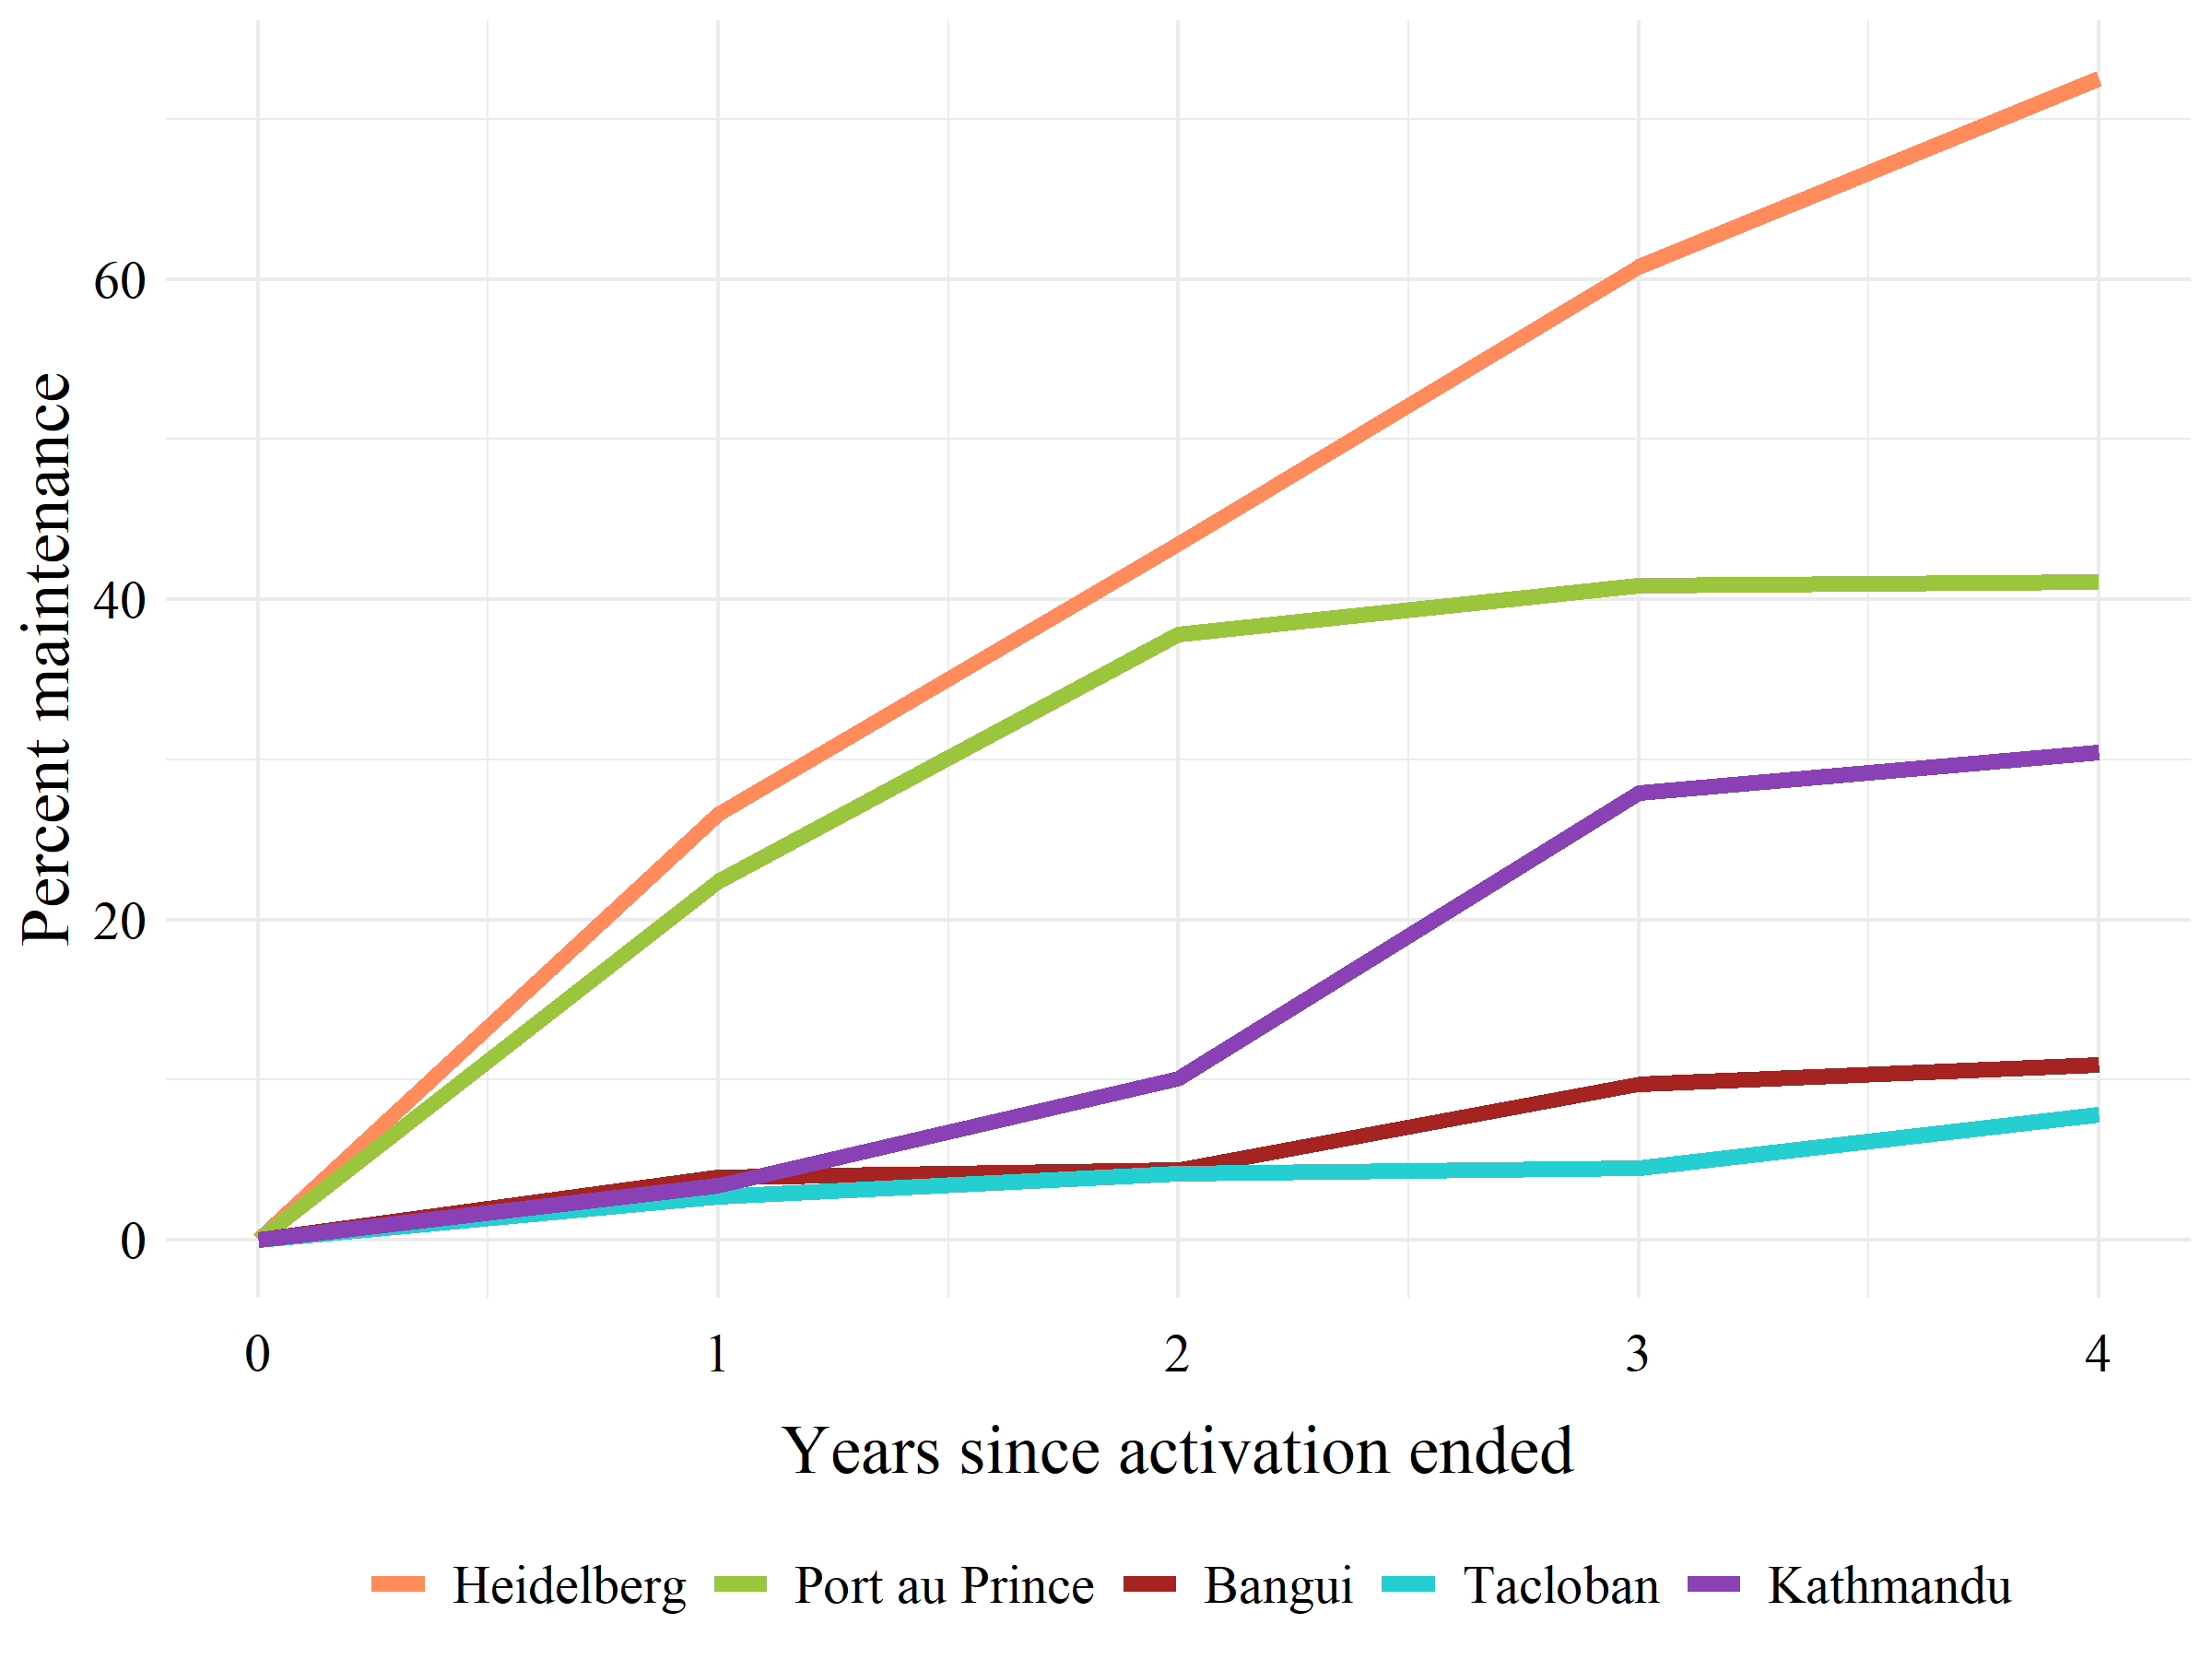
\includegraphics[width = \textwidth]{Images/totmaint.png} %this tells latex what graphics to include. 
    \caption[Percent of total maintained data over time.]{Cumulative percentage of maintained data (deleted or modified at least once) in years following end of mapping campaign} % this prints the caption below the figure
    \label{fig:tot} % this internally labels the figure for future referencing.
\end{figure}
%%%%%%%%%%%%%%%%%%%%%%%%%% 

Figure \ref{fig:tot}, above, provides an initial look at the prevalence of data maintenance in each case study. This figure shows the cumulative percentage of features, created during the mapping campaign period, that have been modified at least once in the years after the campaign has ended. I note that this and all subsequent figures include entity deletion within the definition of maintenance. 

I see that the reference case study, Heidelberg, has a significantly higher prevalence of data maintenance, as over 70\% of this data has been modified or deleted in the four years after it was originally created. Among the humanitarian case studies, the Port au Prince and Kathmandu campaigns stand out for both reaching above 30\% maintenance by the end of this four-year period. The other humanitarian case studies in Tacloban and Bangui only reach approximately 10\% maintenance during this time. Figure \ref{fig:tot} also shows how the rate of maintenance in Heidelberg appears to be approximately consistent during this time period, while maintenance efforts in the humanitarian case studies have plateaued in the fourth year after the campaign has ended. Maintenance efforts in Kathmandu increased notably in the third year after the campaign ended.

%%%%%%%%%%%%%%%%%%%%%%%%%% Distribution of maintenance
\begin{figure} % opens the figure environment. the '[H]' forces the image to be Here
    \centering % puts the image in the horizontal centre of the page
    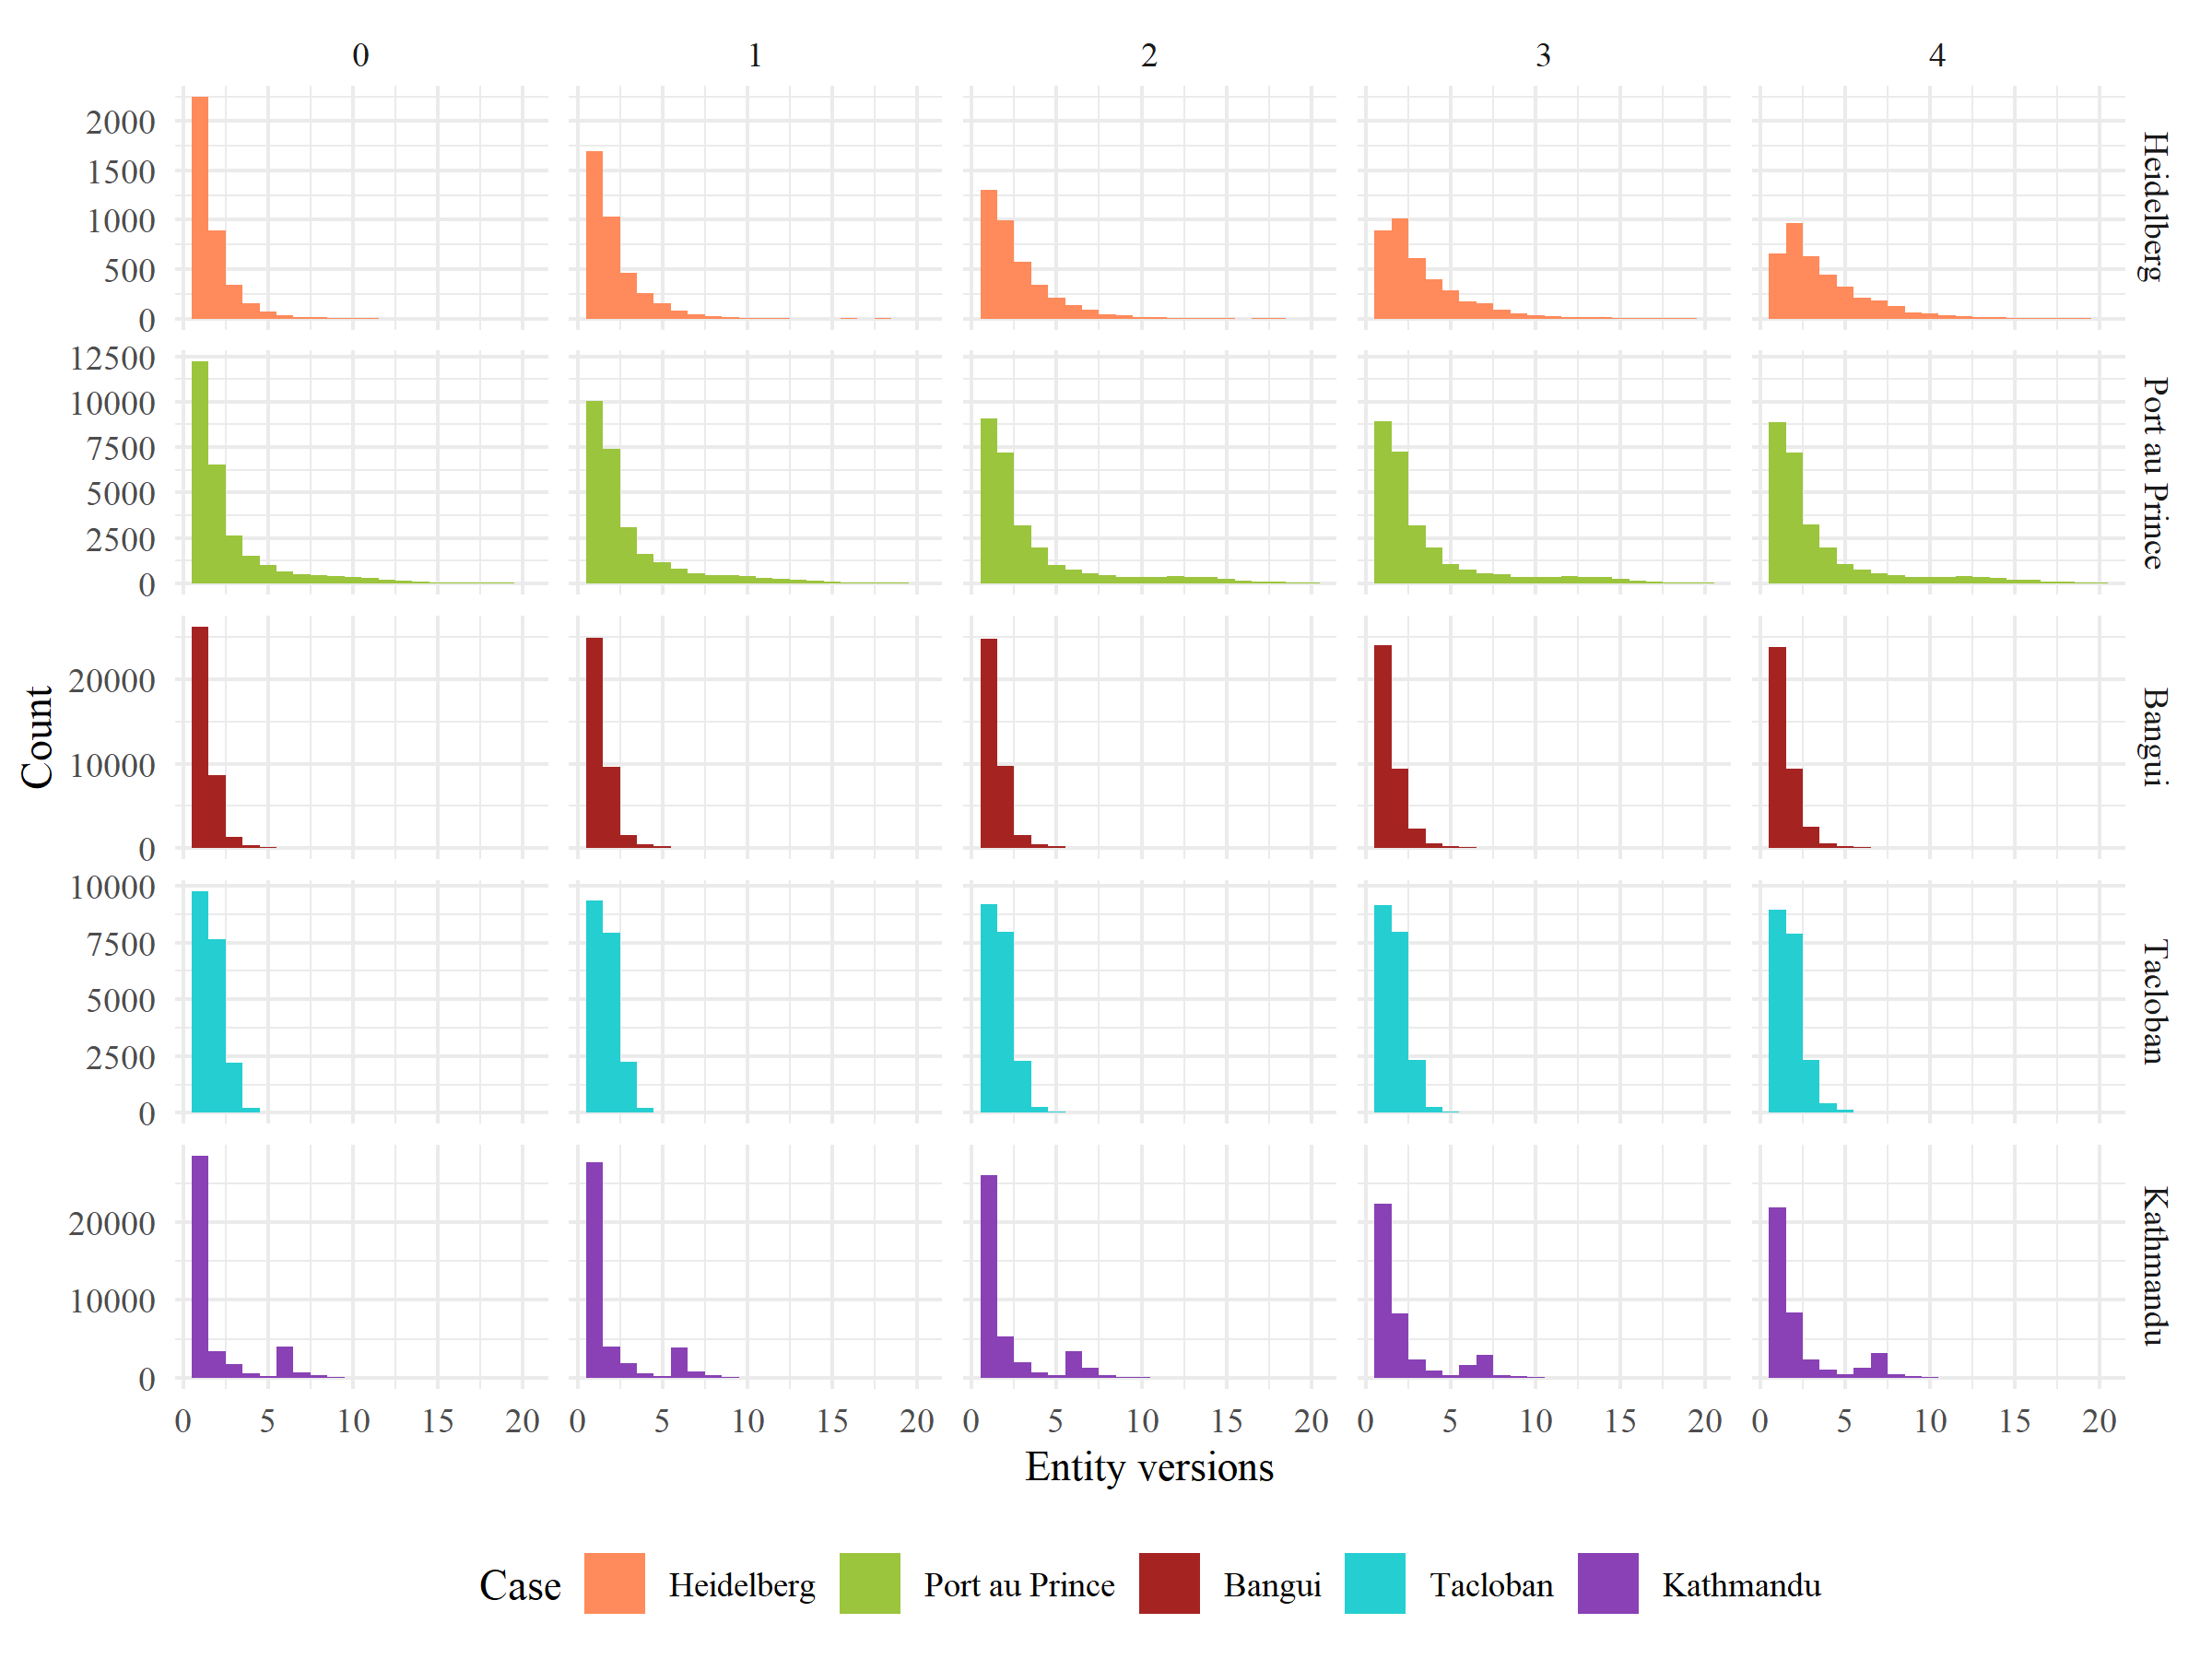
\includegraphics[width = \textwidth]{Images/facetmaint.png} %this tells latex what graphics to include. 
    \caption[Distribution of maintenance frequency for features created during each case study.]{Distribution of maintenance frequency for features created during each case study, from 1-4 years (cumulatively) since the end of each campaign.} % this prints the caption below the figure
    \label{fig:dist} % this internally labels the figure for future referencing.
\end{figure}
%%%%%%%%%%%%%%%%%%%%%%%%%% 

In Figure \ref{fig:dist} I consider data maintenance efforts by looking at the distribution in the maintenance frequency over time of all features that were created during each campaign. The x-axis of this figure is broken down by cumulative number of years since the end of the mapping campaign, and the y-axis is broken down by case study. In the first year after each mapping campaign, I see that the majority of features in all case studies have never been maintained. Changes in the distribution of maintenance frequency are the most noticeable in the Heidelberg reference case, where the passing of time leads to a distribution that is less positively skewed, and towards higher frequency of maintenance in features. After four years, many features have been maintained more than once, with the majority of features classified within the \textit{moderate} category (3-10 versions). Conversely, across all humanitarian cases, I see that the majority of features have still not been maintained after four years has passed. However, as is also reflected in Figure \ref{fig:tot}, the data from the Port au Prince and Kathmandu campaigns has been more frequently maintained than the other humanitarian cases. 

Figures \ref{fig:types} and \ref{fig:feats} illustrate the maintenance frequency distribution for features from each case study after four years have passed since the end of the mapping campaign. Figure \ref{fig:types} is disaggregated to show differences between node and way data types, and Figure \ref{fig:feats} is disaggregated to show differences between features that are tagged with the \texttt{building}, \texttt{highway}, and all other tags. In Figure \ref{fig:types}, I see that nodes and ways follow roughly the same distribution of maintenance frequency across case studies. I see similar results in Figure \ref{fig:feats}. Interestingly, however, it appears as though nodes have been relatively well-maintained in the Port au Prince case study. In Kathmandu, the majority of the \textit{other} features have been maintained at least once. Across all cases, I see that buildings are the most poorly maintained feature. 

%%%%%%%%%%%%%%%%%%%%%%%%%% Distribution of maintenance
\begin{figure} % opens the figure environment. the '[H]' forces the image to be Here
    \centering % puts the image in the horizontal centre of the page
    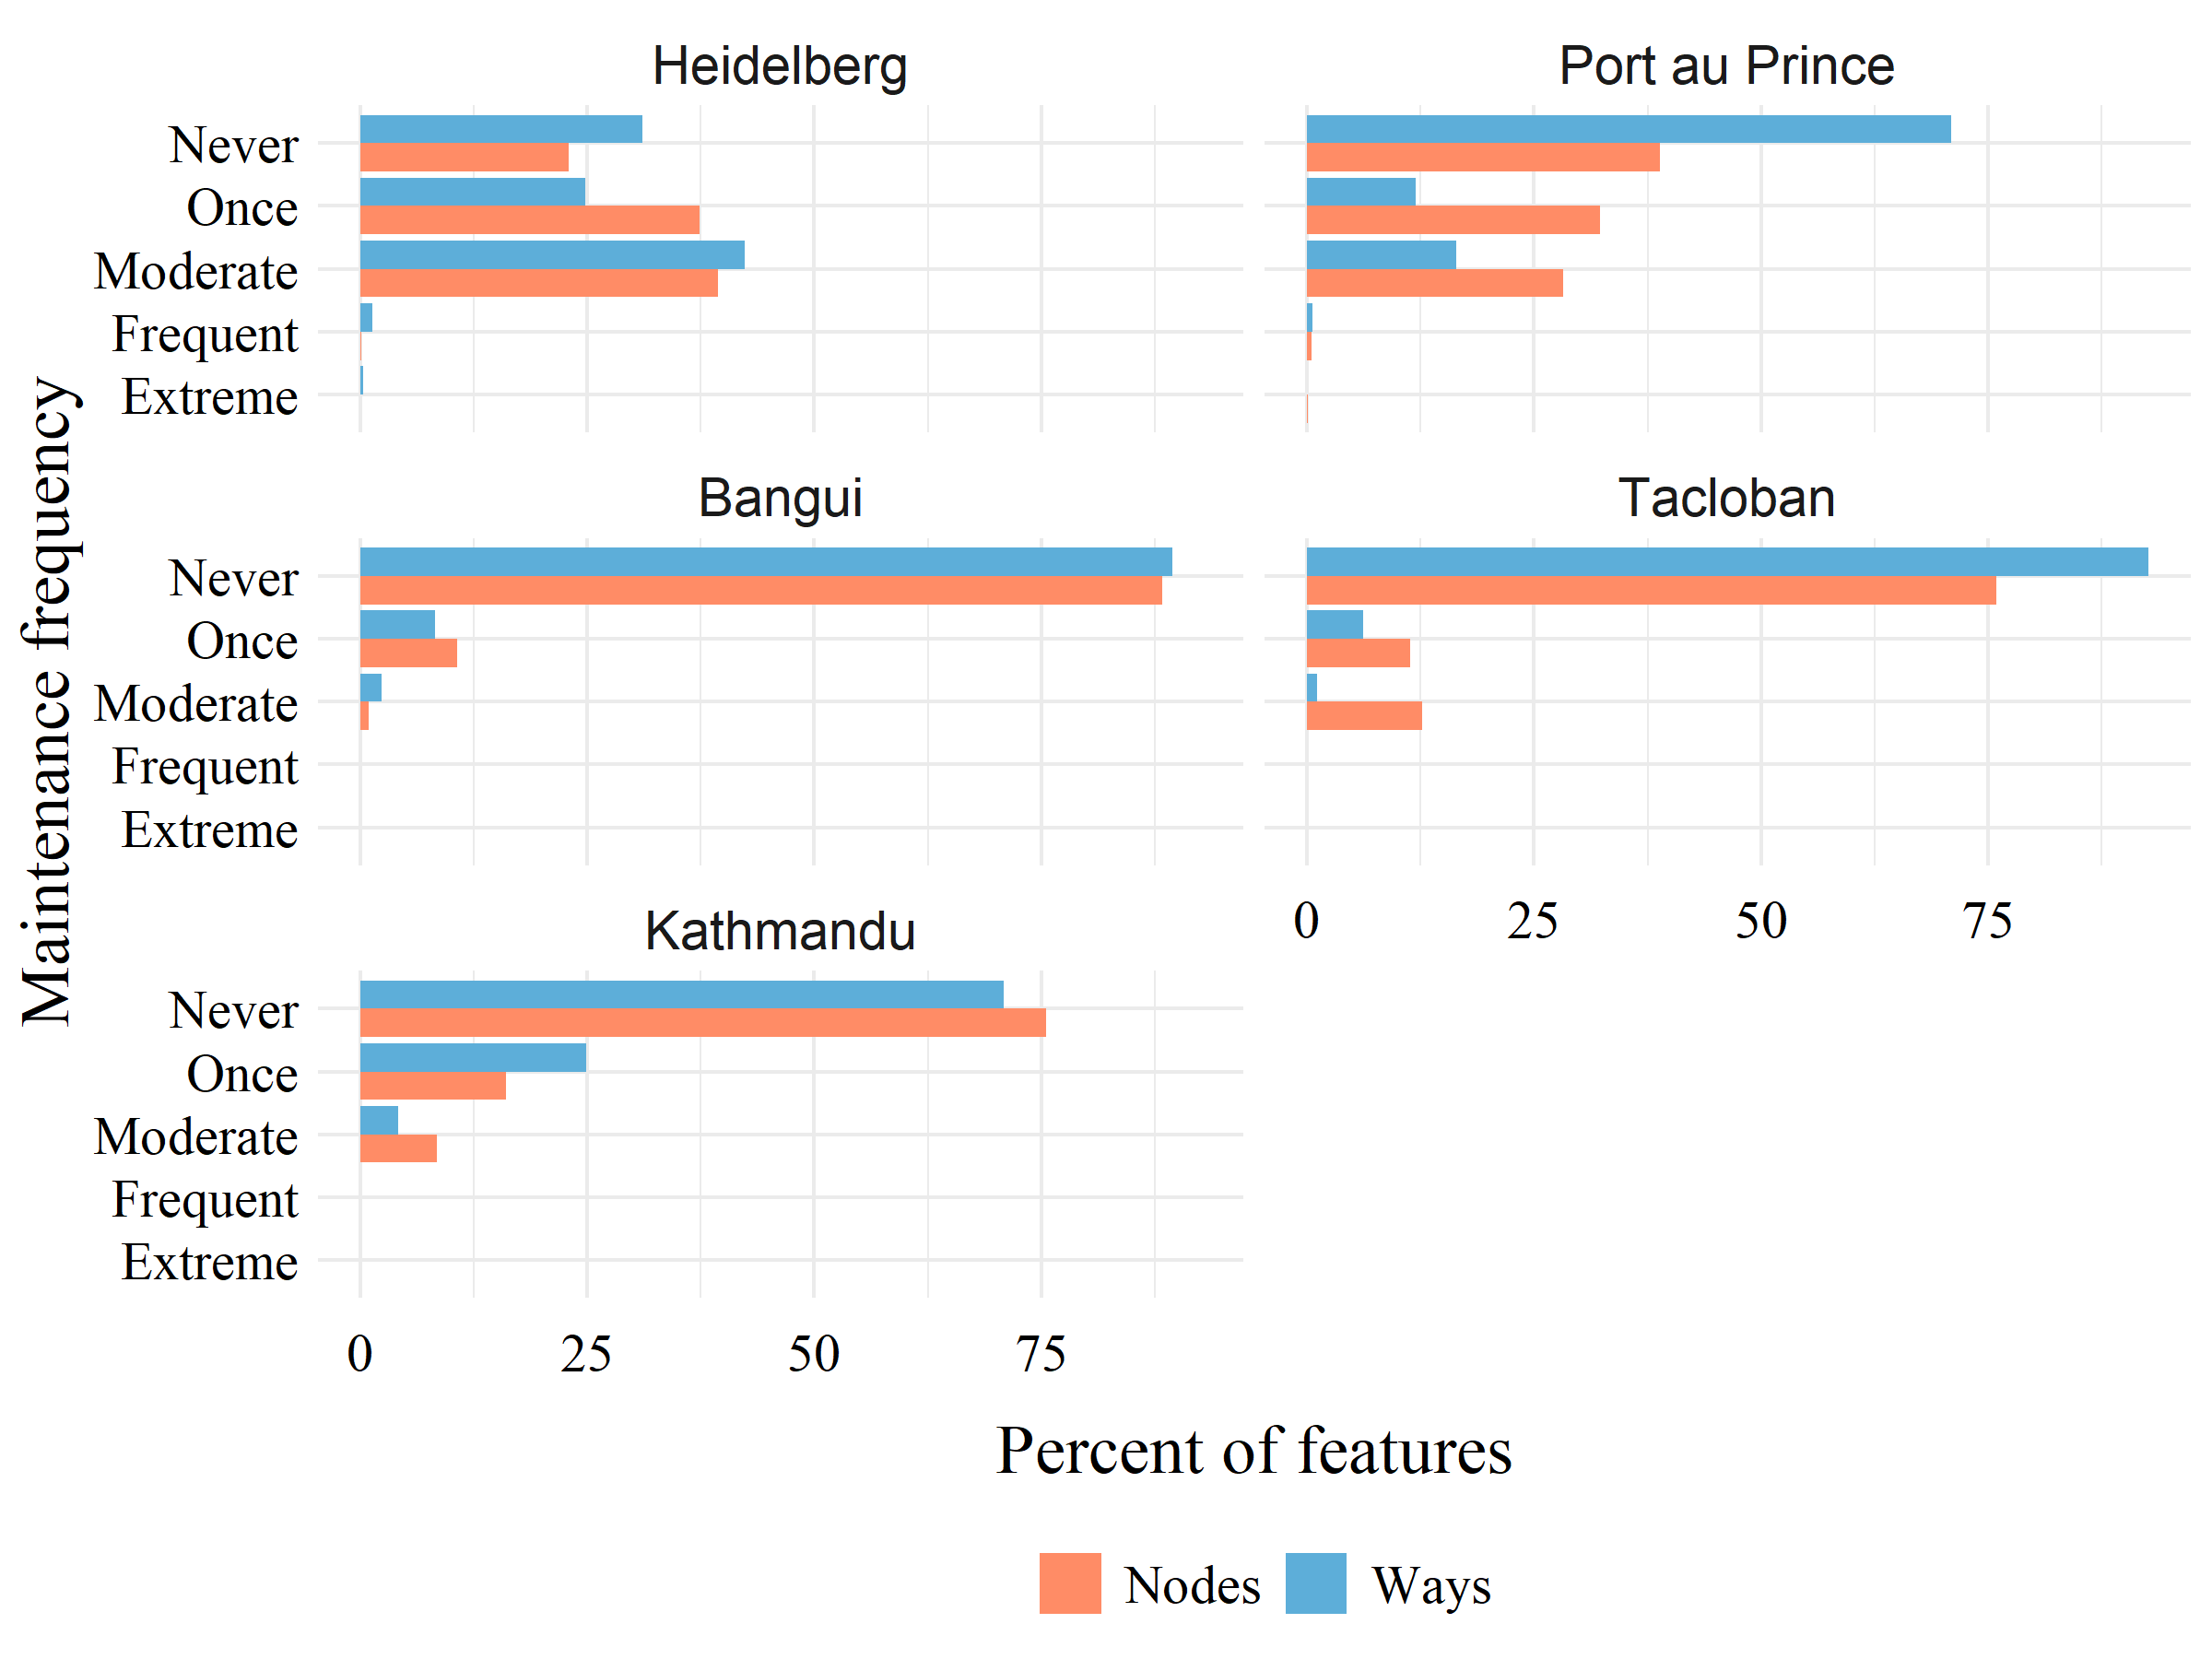
\includegraphics[width = \textwidth]{Images/typesmaint.png} %this tells latex what graphics to include. 
    \caption{Maintenance frequency of nodes and ways for each case study, four years following the end of each mapping campaign.} % this prints the caption below the figure
    \label{fig:types} % this internally labels the figure for future referencing.
\end{figure}
%%%%%%%%%%%%%%%%%%%%%%%%%% 

%%%%%%%%%%%%%%%%%%%%%%%%%% Distribution of maintenance
\begin{figure} % opens the figure environment. the '[H]' forces the image to be Here
    \centering % puts the image in the horizontal centre of the page
    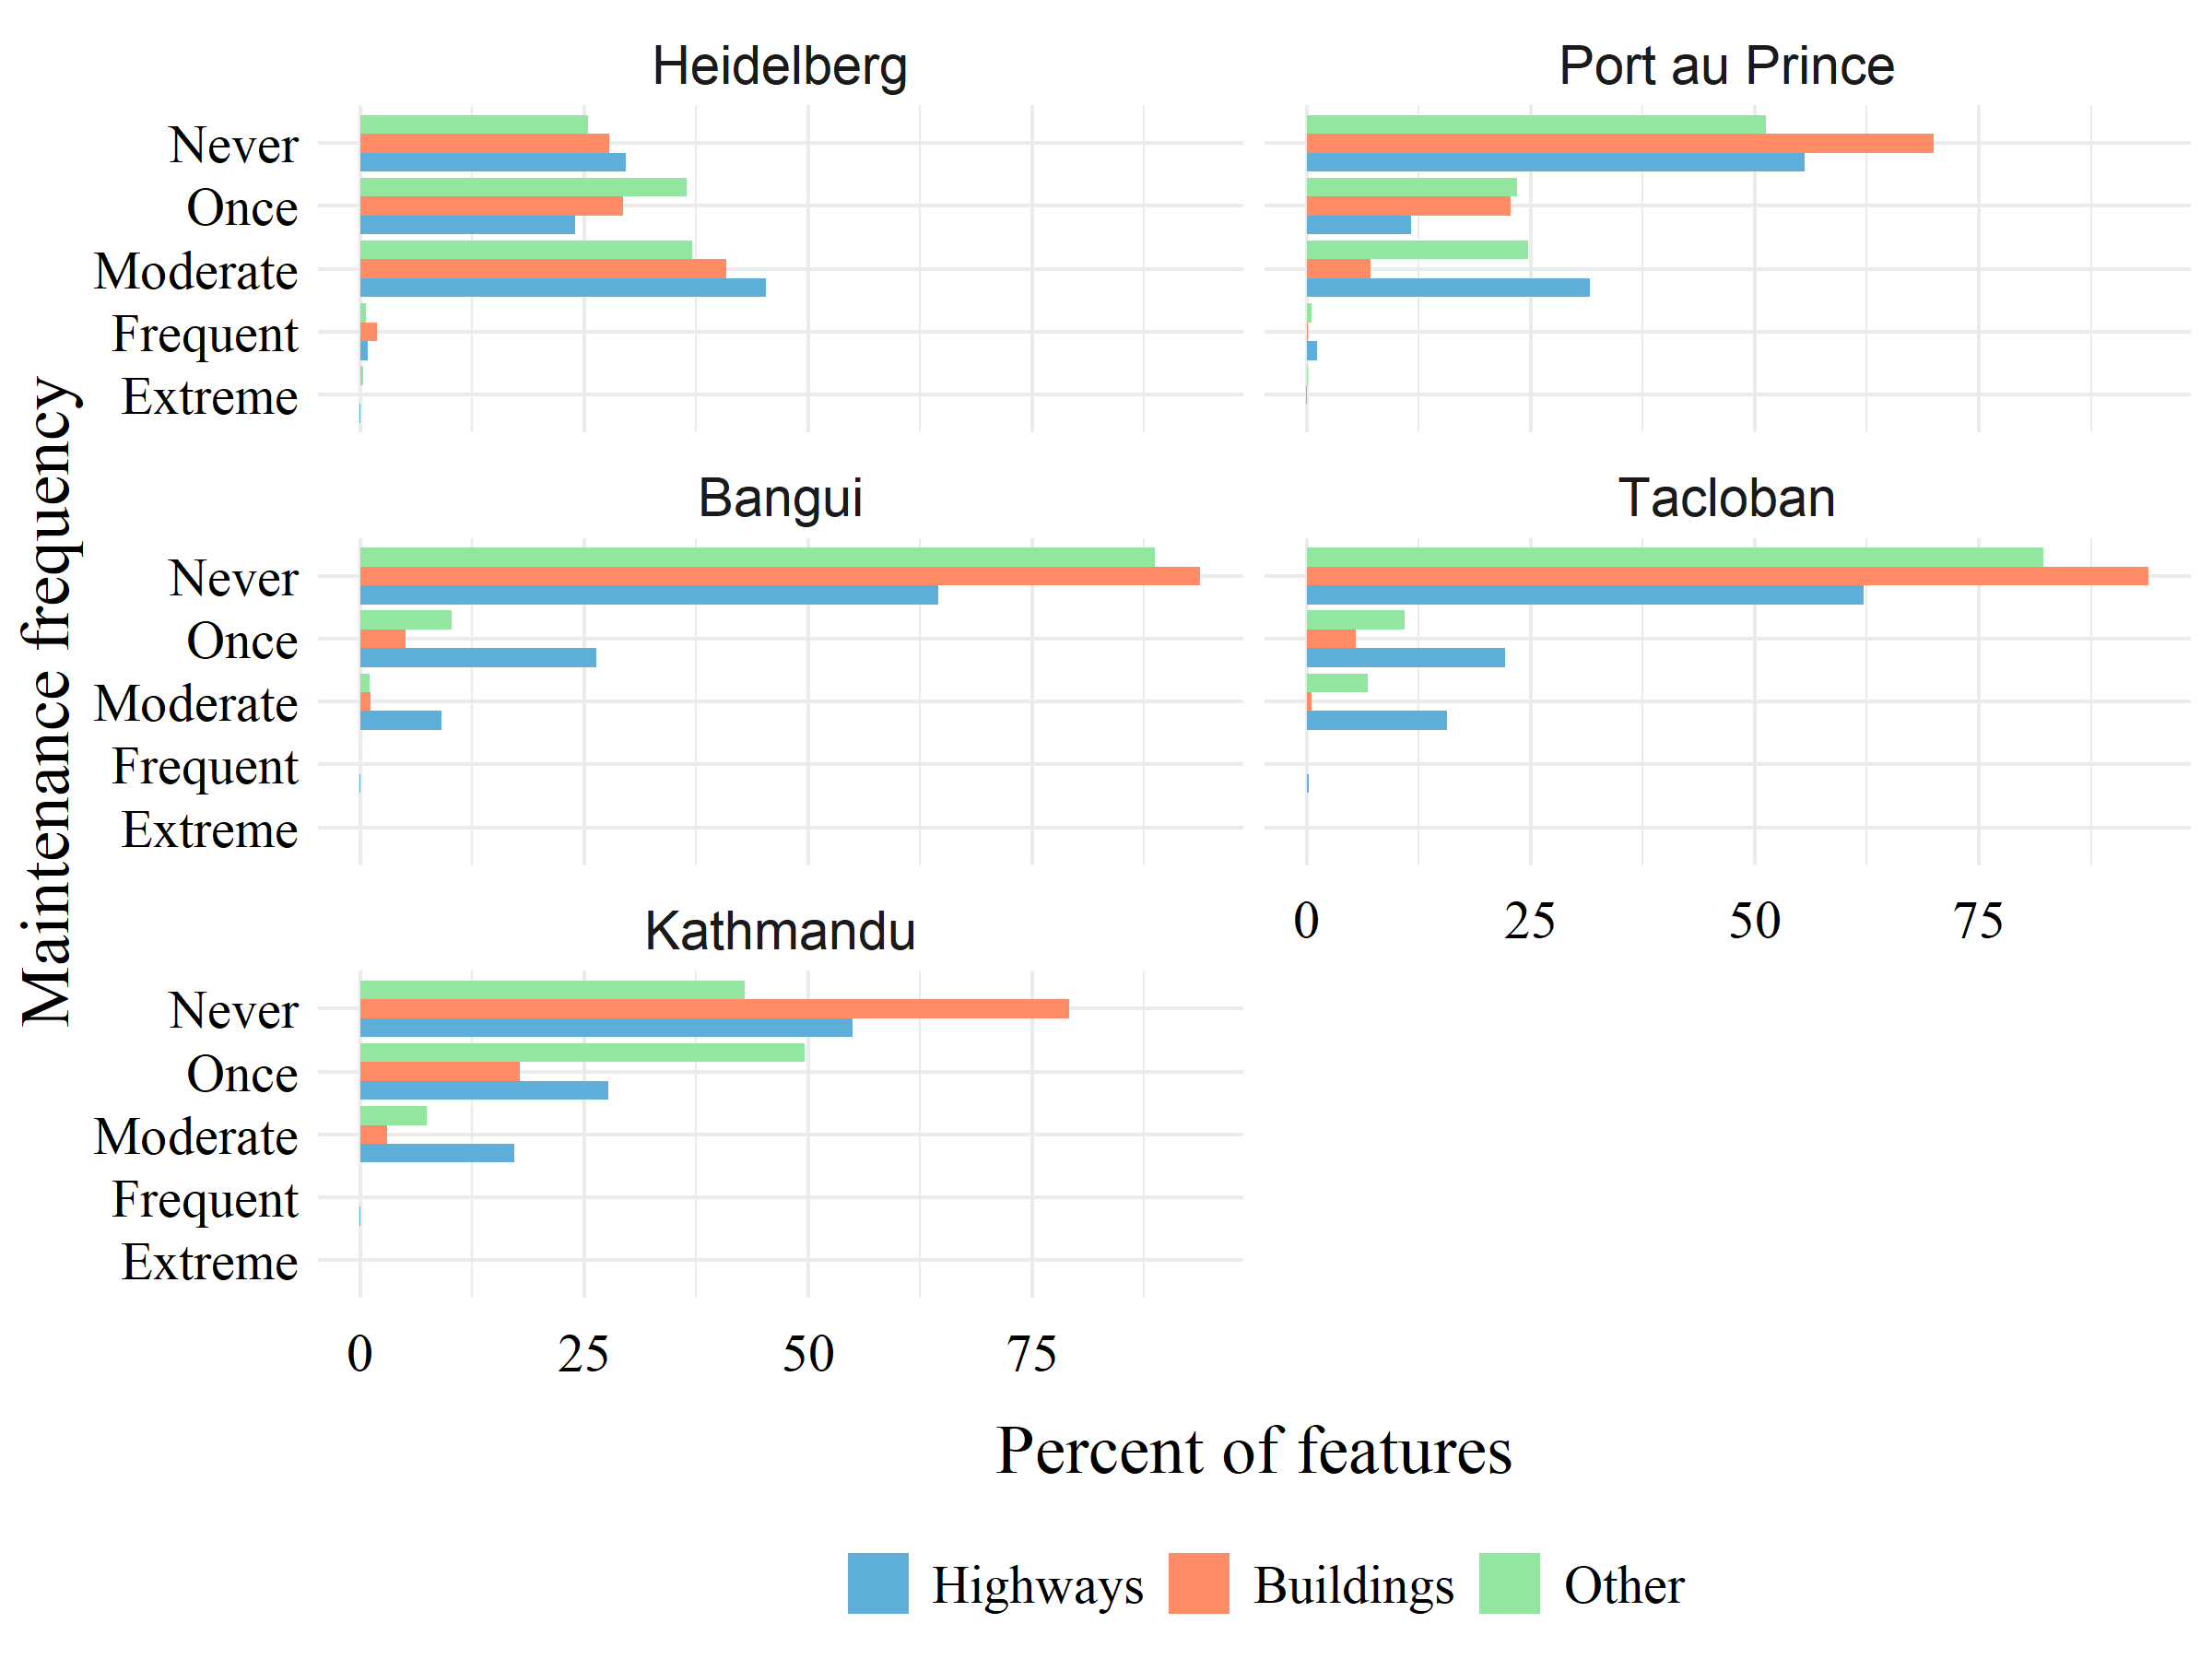
\includegraphics[width = \textwidth]{Images/featmaint.png} %this tells latex what graphics to include. 
    \caption[Maintenance frequency of features with \texttt{building}, \texttt{highway}, and all other tags for each case study.]{Maintenance frequency of features with \texttt{building}, \texttt{highway}, and all other tags for each case study; four years following the end of each mapping campaign.} % this prints the caption below the figure
    \label{fig:feats} % this internally labels the figure for future referencing.
\end{figure}
%%%%%%%%%%%%%%%%%%%%%%%%%%

